\section{Alignment marks}\label{alignment_marks_chapter}

The very first thing which has to be done when receiving a bunch of new wafers from the supplier, is to clean them with hot sulfuric acid
and to remove native oxide on top, by dipping it into HF. The time for the HF dip depends on the concentration.

After that one has to etch some kind of alignment marks into the silicon, which allows the stepper to match the different mask layers
to each other during exposure.

\begin{figure}[H]
	\centering
	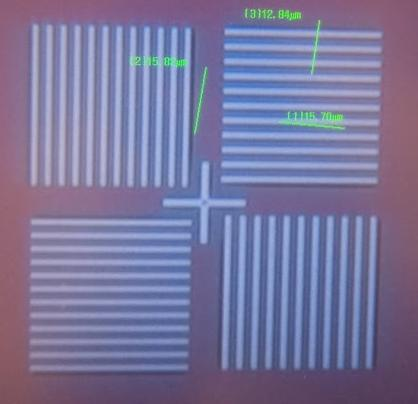
\includegraphics[scale=0.5]{pictures/alignment_cross.png}
	\caption{Picture of an alignment mark}
	\label{alignment_mark_target}
\end{figure}

How such an alignment mark might look like is being shown in \autoref{alignment_mark_target}, which is the ASML mark used for the ASML stepper units.

Depending on the alignment strategy there can be two or more alignment marks being etched into the substrate, and the positioning entirerly depends on
the pattern recognition software and alignment strategy of the specific machine.

The depth of this silicon etching is usually around 200nm or so, but is nothing really critical to support LibreSilicon but more something stepper
aligner specific.

The manufacturer of the stepper aligner usually provides pre made masks for this step and provide requirements for the depth of those marks inside the
silicon.

The ASML stepper has two alignment marks left and right of the wafer, which, when connected to a line, are in parallel to the notch.

Those marks are critical for aligning the patterns correctly above each other during all the further manufacturing steps, so it should be taken care,
that those markers stay always visible, so that the machine can find them and orient itself on it.
